\section{Pseudoalignment}\label{sec:Pseudoalignment}

\subsection{Background}

To start describing pseudoalignment, colored DBG must be described first~\cite{CDBG, SuccinctColoredDeBruijnGraphs}.
Throughout this chapter and beyond, the terms $u64$, $u8$, and other variants may be used.
$u64$ means an unsigned 64-bit integer, whereas $u8$ means an unsigned 8-bit integer, and so on for other values of this format.
Lets take a look at Figure~\ref{fig:FastaqToCdbg}.
Say that you are given 2 sequences $S_1$ and $S_2$ with $k$-mer sets $K_1 = a_1, a_2, \ldots, a_n$ and $K_2 = b_1, b_2, \ldots, b_m$.
Now each sequence is given a label, usually some u64.
If a $k$-mer belongs to a sequence, the $k$-mer is marked with the same label as the sequence.
Moreover, if a $k$-mer belongs to multiple sequences, it is marked with the label of that sequence.
These labels are the colors.
Implementation-wise, these colors are represented as simple u64s, so each $k$-mer has a set of u64s associated with it~\cite{Themisto}.

\begin{figure}[t]
  \centering
  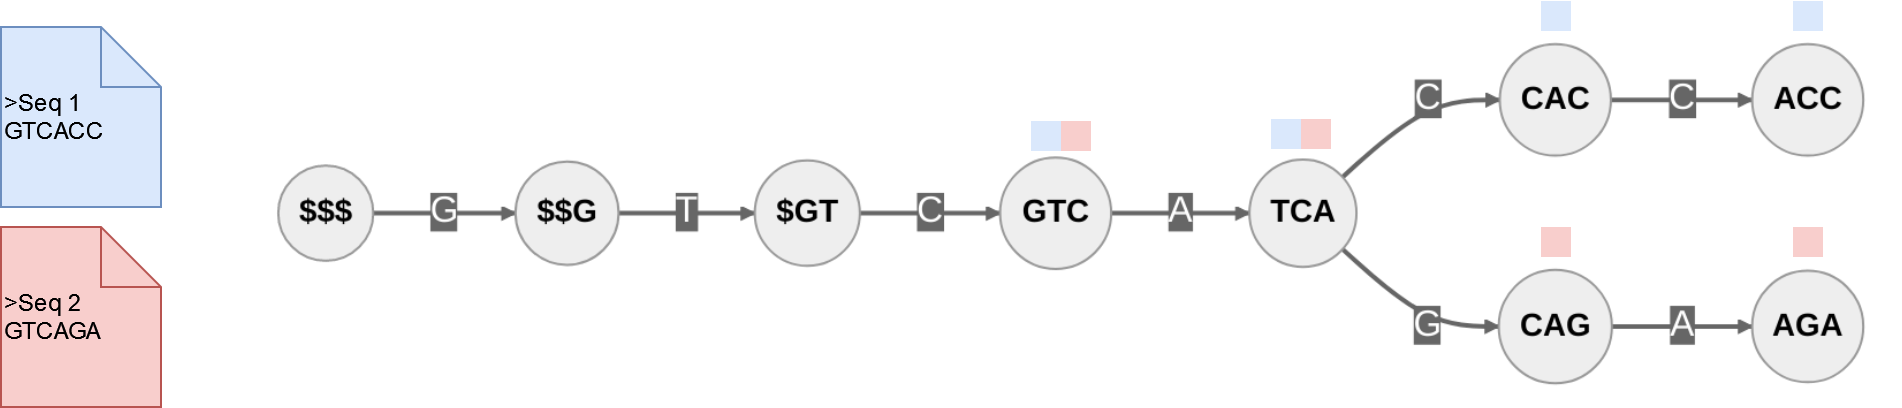
\includegraphics[width=\textwidth]{images/FastaqToCdbg.png}
  \caption{Transforming FASTA/FASTQ files into a colored DBG with $k=3$. Reverse complements are not included in this example.}\label{fig:FastaqToCdbg}
\end{figure}

Different sequences may have the same color.
One use of this is to group the sequences of a single reference genome and say they all have the same color.
This way, if a $k$-mer is labeled with the color of a reference genome, it is known that the $k$-mer is found in that genome.
Then, if all the color sets of all $k$-mers of a read contain the same color, that is, the intersection of all the color sets has a color, one may say that the read is found in the reference genome associated with that color.
If a $k$-mer is not found in the DBG, then it is ignored.
This is the technique used by Kallisto~\cite{Kallisto}, the first pseudoalignment tool.

Metagraph~\cite{Metagraph} and Bifrost~\cite{Bifrost}, two separate pseudoalignment tools, went one step further than Kallisto and instead of ignoring the $k$-mers not found in the DBG, they set a threshold $\tau$, and if more than $\tau$ color sets of $k$-mers in a read include a color, then it is said that the read is associated with that color.
$\tau$ is percentage based, not a discrete threshold.
Themisto~\cite{Themisto}, whose implementation this work is based on, combines the two methods so that the user can choose to remove or include the $k$-mers with no color sets, and then set a threshold on the remaining $k$-mers.
If a threshold $\tau=1.0$ is set and the missing $k$-mers are ignored, then the result is the same as Kallisto.
Meanwhile, if the missing $k$-mers are included, the results are the same as those of Metagraph and Bifrost~\cite{Themisto}.
Themisto has shown to be the best method as, besides supporting both threshold and the removal of missing $k$-mers, it is usually faster and uses less space than other methods~\cite{Themisto}.
Metagraph has the potential of using less memory for its index when using binary-relation wavelet trees, but then has 100 times less query throughput on some datasets~\cite{Themisto}.

When doing pseudoalignment, a DBG is usually built out of the $k$-mers of many reference genomes, and each $k$-mer is given the colors of all genomes it belongs to.
Thus, there are as many colors as genomes within this DBG.
However, if the dataset has hundreds of thousands of genomes, it may be a good idea to group some of them together, thus avoiding having too many colors, as this may lead to intense memory requirements and processing times, especially if each $k$-mer has its own color set.
Pseudoalignment works because it was found that it is often not necessary to know in which position a read was within a genome to attribute it to a genome, only which genome it originated from~\cite{Kallisto}.

\subsection{Themisto}

Now, the construction and optimisations of the colored DBG as used in Themisto~\cite{Themisto}, which uses GGCAT~\cite{GGCAT} for colored unitig construction, will be discussed.
Firstly, there is no need to keep a color set for every $k$-mer.
Rather, certain conditions can be identified where the $k$-mers must have an associated color set, and for the rest of the $k$-mers the algorithm would need to move forward in the graph until the next $k$-mer which has a color set.
If two $k$-mers have the same color set, they can point to the same memory position, rather than duplicating the colors, hence avoiding doubling memory requirements.
The $k$-mers with a color set associated with them are called key-$k$-mers.
The conditions for a vertex to be labeled as a key-$k$-mer, and therefore must have a color set associated with it, are described next, and visualised in Figure~\ref{fig:KeyKmers}.
Reference is made to this figure as each condition is described.

The first condition out of four for being a key-$k$-mer is if it is outgoing to another vertex which is the first $k$-mer from a reference sequence.
This condition causes the vertex with $k$-mer \textit{CTT} to be a key-$k$-mer.
The second condition is if it is the last $k$-mer of a reference sequence.
This condition causes $k$-mers \textit{CCT, CGG} and \textit{GAG} to be key-$k$-mers.
Third, if it has an outgoing edge to a vertex $v_i$ with $\#in_v(v_i) \ge 2$.
Because of this, \textit{TAC} and \textit{AAC} are labeled as key-$k$-mers.
Fourth and last, if the vertex $v_i$ itself has $\#out_v(v_i) \ge 2$.
The last condition causes \textit{TCG} to be labeled as a key-$k$-mer.
Notice how each unitig will have the same color set, unless a new sequence starts or ends in the middle of that unitig.

Remember that these rules exist because one can always go forwards in the graph, using Algorithm~\ref{alg:MovingForward}, but not backwards.
This algorithm assumes a single outgoing edge from the current vertex, otherwise, it would lead to ambiguities.
The less steps needed, the better, because for each step in the graph walk that needs to happen requires a random read, since the $k$-mers are not ordered by their position in the graph, but colexicographically based on their $k$-mers.
As a result, ideally, every vertex would be a key-$k$-mer, which means that the color set for each $k$-mer would be stored.
However this causes too much memory to be used, as it would be necessary to store a pointer for each $k$-mer.
Hence why checkpointing is used, with a parameter $d$, where every d $k$-mers of a uniquely colored unitig becomes a key-$k$-mer.
If $d=1$, this means that every $k$-mer is a key-$k$-mer.
In Chapter~\ref{ch:Results}, the datasets used for this thesis are evaluated with $d=1$ and $d=20$.

\begin{figure}[t]
  \centering
  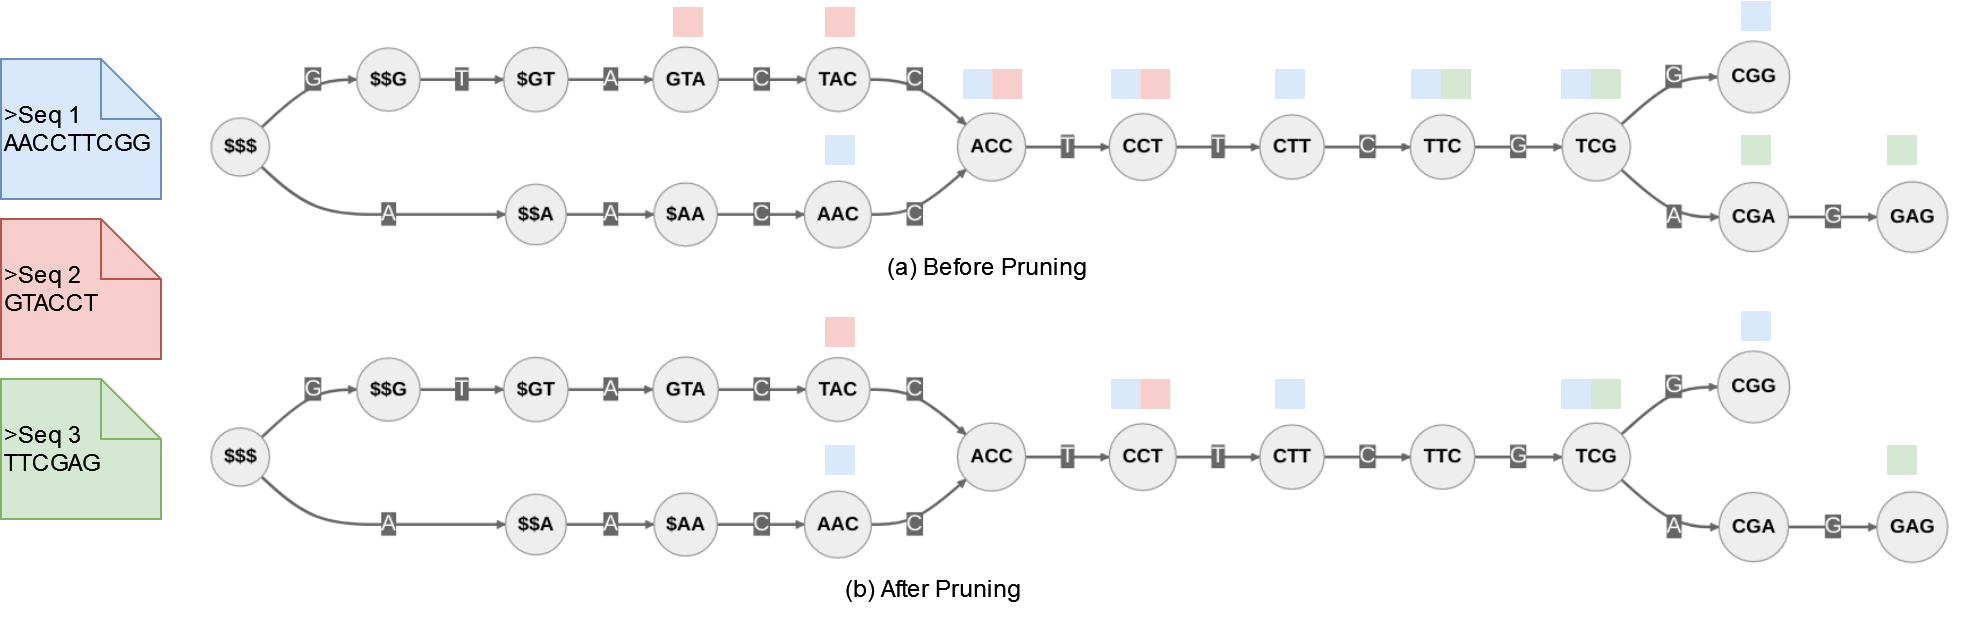
\includegraphics[width=\textwidth]{images/KeyKmers.png}
  \caption{Transforming FASTA/FASTQ files into a colored DBG with $k=3$ and then pruning it for key-$k$-mers. Once more reverse complements are omitted for simplicity of the example, but these would be included also in practice.}\label{fig:KeyKmers}
\end{figure}

\begin{algorithm}
	\KwIn{ \newline
    The current index $i$ \newline
    Bitvectors $b_A, b_C, b_G, b_T$ \newline
    c-map $C$
	}

  \ForEach{$b$ \textbf{in} $Bitvectors$}{\
    \If{$b$ = 1}{\
      \textbf{return} $C[label]$ + rank($b, i$)
    }
  }
	\caption{Walking 1 step forward in the SBWT}\label{alg:MovingForward}
\end{algorithm}

Next the color set storage in Themisto is discussed.
Figure~\ref{fig:ColorComponents} contains a visualisation of each of the components which makes up the whole color structure.
First is a bitvector indicating the key-$k$-mers, the \textit{key\_kmer\_marks}, where a 1 at index $i$ indicates that the vertex at index $i$ corresponds to a key-$k$-mer.
The length of this bitvector is the same length as the number of vertices.
Next, there is the color set indexes \textit{color\_set\_idxs}, which are integers that point key-$k$-mers to the index of the color set they are associated with.
Additionally, a bitvector of the same size of the \textit{key\_kmer\_marks} indicates how the color set for that $k$-mer is stored, the \textit{is\_dense\_marks}.

Themisto uses an adaptive color set storage method which allows it to save a lot of space, which is called the \textit{hybrid} technique.
Using this method, there are two ways a color set can be stored: dense or sparse.
The dense method stores color sets as bitvectors, where a 1 indicates that the color at that index is present.
Any trailing 0s are truncated as an optimisation.
The bitvectors for the dense color sets are stored contiguously in a large bitvector called the \textit{dense\_arrays}.
Thus, another vector of unsigned integers is necessary, to indicate at which bit each color set starts and ends, called the \textit{dense\_arrays\_intervals}.
This array has a final unsigned integer at the end that has the end of the last vector, which would be the start of the next bitvector if it existed.
A compact vector of unsigned integers is used.
Compact means that the vector uses only as much memory as needed, by using $\lceil log_2(n) \rceil$ bits per character, where $n$ is the largest index.
The sparse format then uses compact vectors to store the color set indexes which are present in a color set, the \textit{sparse\_arrays}.
Similarly to the dense format, the sparse vector is stored contiguously, so another compact vector is used to store the start indexes, dubbed as the \textit{sparse\_arrays\_intervals}.
Each sub-array in the \textit{sparse\_arrays} is sorted, to make querying and therefore intersecting the color sets of reads later easier.

\begin{figure}[t]
  \centering
  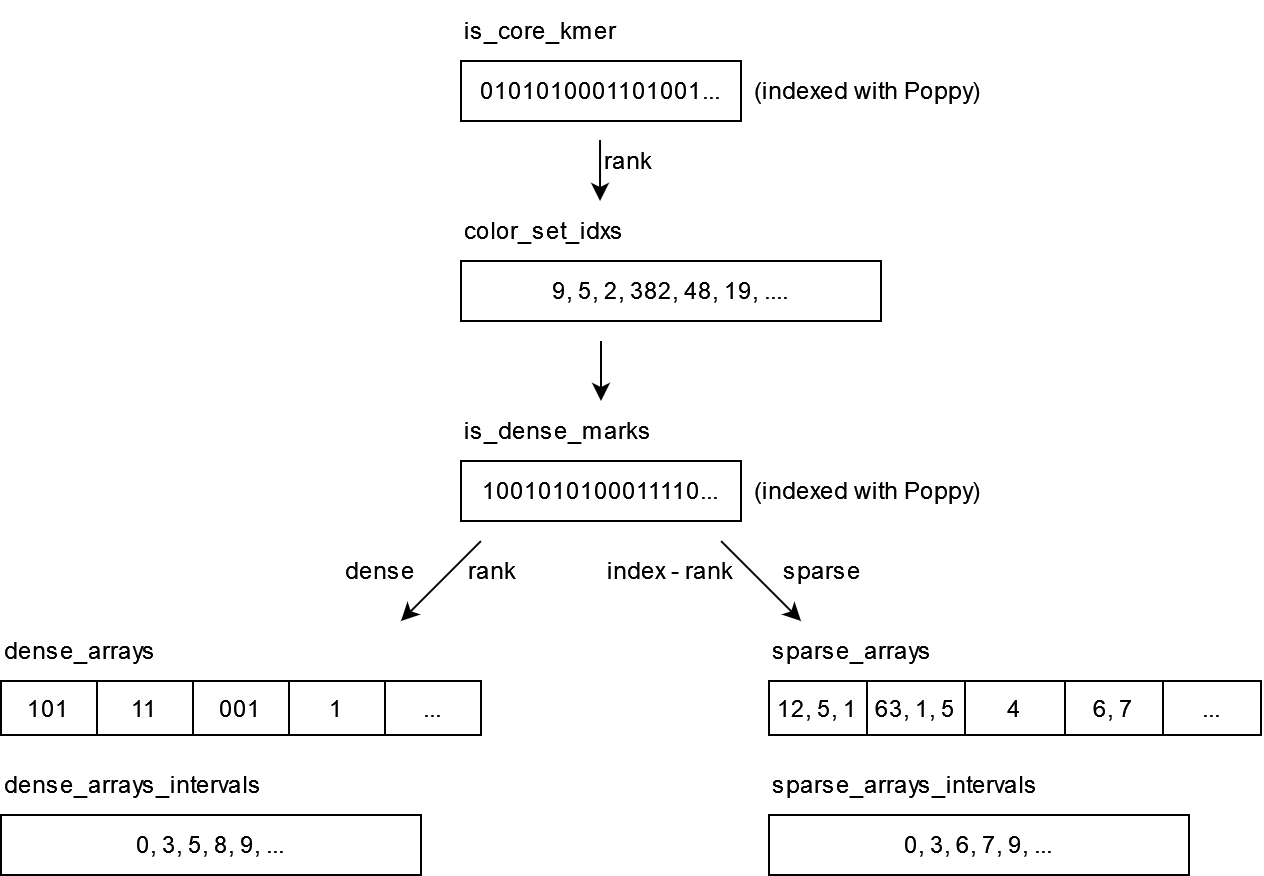
\includegraphics[width=0.85\textwidth]{images/ColorComponents.png}
  \caption{A visualisations of all components used for color storage and some hints for searching. Note that all non-bitvector arrays are compact unsigned integer vectors.}\label{fig:ColorComponents}
\end{figure}

Algorithm~\ref{alg:ColorSearch} shows the color set search, given the index of a key-$k$-mer.
This corresponds to Figure~\ref{fig:ColorComponents} and the terminology used so far, which will carry on to the next section as well.
Themisto uses some optimisations for combining color sets.
For example, when $\tau=1.0$, a technique which is also used in Kallisto~\cite{Kallisto}, is that when both color sets that need to be combined are dense, a bitwise AND can be used.

\begin{algorithm}
	\KwIn{ \\
    The index $i$ of a key-$k$-mer in the SBWT structure

    $key\_kmer\_marks$ (indexed with Poppy)

    $color\_set\_idxs$

    $is\_dense\_marks$ (indexed with Poppy)

    $dense\_arrays$

    $dense\_arrays\_intervals$

    $sparse\_arrays$

    $sparse\_arrays\_intervals$

    $num\_colors$
	}

  $color\_set\_idx$ = $color\_set\_idxs[rank(key\_kmer\_marks, i)]$

  $is\_dense$ = $is\_dense\_marks[color\_set\_idx]$

  $is\_dense\_rank$ = rank($is\_dense\_marks, color\_set\_idx$)

  \If{is\_dense}{\
    $start$ = $dense\_arrays\_intervals[is\_dense\_rank]$

    $end$ = $dense\_arrays\_intervals[is\_dense\_rank + 1]$

    \textbf{return} $dense\_arrays[start, \ldots, (end - 1)]$  // returns dense format
  }\Else{
    $start$ = $sparse\_arrays\_intervals[color\_set\_idx - is\_dense\_rank]$

    $end$ = $sparse\_arrays\_intervals[color\_set\_idx - is\_dense\_rank + 1]$

    \textbf{return} $sparse\_arrays[start, \ldots, (end - 1)]$  // returns sparse format
  }

	\caption{Obtaining the color set given the SBWT index and the color structure components.}\label{alg:ColorSearch}
\end{algorithm}

This concludes the background chapter.
The next chapter will discuss the contributions of this thesis to massively parallelise and use all computing resources available to speed up pseudoalignment.
